\documentclass[12pt,a4paper]{report}

\usepackage[utf8]{inputenc}
\usepackage[T1]{fontenc}
\usepackage{lmodern}
\usepackage[top=1in,bottom=1in,left=1.25in,right=1in]{geometry}
\usepackage{graphicx}
\usepackage{amsmath}
\usepackage{amssymb}
\usepackage{setspace}
\usepackage{titlesec}
\usepackage{fancyhdr}
\usepackage{hyperref}
\usepackage{float}
\usepackage{booktabs}
\usepackage{tabularx}
\usepackage{array}
\usepackage{longtable}
\usepackage{enumitem}
\usepackage[table]{xcolor}
\usepackage{tikz}
\usetikzlibrary{arrows.meta,positioning,shapes.geometric,fit,calc}

\hypersetup{colorlinks=true, linkcolor=black, urlcolor=blue, citecolor=blue}
\onehalfspacing
\setlength{\parskip}{4pt}
\setlist[itemize]{leftmargin=18pt}
\setlist[enumerate]{leftmargin=22pt}

\titleformat{\chapter}[display]
  {\normalfont\huge\bfseries\centering}{\chaptertitlename\ \thechapter}{0pt}{\Huge}
\titlespacing*{\chapter}{0pt}{-64pt}{10pt}

\pagestyle{fancy}
\fancyhf{}
\fancyhead[L]{\leftmark}
\fancyfoot[C]{\thepage}
\renewcommand{\headrulewidth}{0.4pt}
\setlength{\headheight}{28pt}

\newcolumntype{Y}{>{\raggedright\arraybackslash}X}
\newcolumntype{C}[1]{>{\centering\arraybackslash}p{#1}}
\newcommand{\coverinforow}[2]{#1 & : & #2\\[0.24cm]}

\begin{document}

\newgeometry{top=0.75in,bottom=0.85in,left=0.85in,right=0.85in}
\begin{titlepage}
    \thispagestyle{empty}
    \begin{singlespace}
    \centering
    \setlength{\fboxrule}{1.1pt}
    \setlength{\fboxsep}{7pt}
    \vspace*{0.10cm}

    {\LARGE Premier University, Chittagong\par}
    \vspace{0.18cm}
    \fbox{\Large Department of Computer Science and Engineering}\par
    \vspace{0.42cm}
    
\includegraphics[width=0.31\textwidth]{logo/puc_logo.png}\\[0.30cm]

    \fbox{\huge\bfseries Final Project Report}\par
    \vspace{0.38cm}

    \begin{flushleft}
        \renewcommand{\arraystretch}{1.20}
        {\large
        \begin{tabularx}{\linewidth}{@{}p{0.29\linewidth}p{0.03\linewidth}X@{}}
            \coverinforow{Course Title}{Software Engineering Laboratory}
            \coverinforow{Course Code}{CSE 3234}
            \coverinforow{Project Title}{Hostel Management System}
            \coverinforow{Academic Year}{2025--2026}
            \coverinforow{Date of Submission}{April 2026}
            \coverinforow{Session}{Fall 2025}
        \end{tabularx}
        }
    \end{flushleft}

    \vspace{0.32cm}
    \rule{\linewidth}{0.4pt}
    \vspace{0.32cm}

    \noindent
    \fbox{%
    \begin{minipage}[t][4.4cm][t]{0.41\linewidth}
        \raggedright
        {\Large\bfseries Submitted To :\par}
        \vspace{0.30cm}
        {\Large\bfseries Estiak Ahamed Sazid\par}
        \vspace{0.36cm}
        {\large Lecturer\par}
        {\large Department of Computer Science and Engineering\par}
        {\large Premier University, Chittagong}
    \end{minipage}}
    \hfill
    \fbox{%
    \begin{minipage}[t][4.4cm][t]{0.51\linewidth}
        \raggedright
        {\Large\bfseries Submitted By :\par}
        \vspace{0.36cm}
        {\large
        \renewcommand{\arraystretch}{1.16}
        \begin{tabularx}{\linewidth}{@{}Xr@{}}
            Srabonti Dey & 0222310005101001\\
            Ismat Fariha Any & 0222310005101025\\
            Md Jahedul Islam & 0222310005101037\\
            Md Kamrul Islam & 0222310005101039\\
        \end{tabularx}
        \vspace{0.2cm}
        43th Batch, 6th Semester, B1 Section\par
        }
    \end{minipage}}
    \end{singlespace}
\end{titlepage}
\restoregeometry

\pagenumbering{roman}
\tableofcontents
\newpage
\cleardoublepage
\pagenumbering{arabic}

\chapter{Introduction}
\section{Introduction}
The Hostel Management System is a web-based software project developed to manage hostel meal, billing, complaint, notice, and administrative activities from a single platform. The project separates user responsibilities into student, manager, and administrator roles so that each user sees only the features needed for their work.

\section{Motivation}
Manual hostel management often depends on paper records, message groups, and verbal communication. This can cause incorrect meal counts, delayed notices, billing confusion, and weak complaint tracking. A digital system can reduce these problems by storing information in a structured and traceable way.

\section{Objectives}
\begin{enumerate}
    \item To provide a digital platform for hostel service management.
    \item To support role-based access for students, managers, and administrators.
    \item To make meal planning, attendance, billing, notices, and complaints easier to monitor.
\end{enumerate}

\chapter{Software Requirements Specification}
\section{Functional Requirements}
\begin{itemize}
    \item Users shall be able to register and log in securely.
    \item Students shall be able to view menus, submit meal choices, check bills, and submit complaints.
    \item Managers shall be able to manage menus, attendance, and inventory.
    \item Administrators shall be able to manage users, billing, notices, analytics, and settings.
\end{itemize}

\section{Non-functional Requirements}
\begin{itemize}
    \item The system should be responsive on desktop and mobile browsers.
    \item Passwords should be stored securely using hashing.
    \item The backend should validate user input and protect private routes.
    \item The codebase should be modular so that future features can be added easily.
\end{itemize}

\chapter{Methodology}
\section{Architecture}
The project follows a client-server architecture. The frontend communicates with a backend API, and the backend stores persistent data in a database. Authentication middleware protects role-specific routes.

\begin{figure}[H]
\centering
\begin{tikzpicture}[
  node distance=1.6cm,
  box/.style={draw, rounded corners, align=center, minimum width=3.2cm, minimum height=1cm},
  arrow/.style={-Latex, thick}
]
\node[box] (client) {Frontend\\React UI};
\node[box, right=of client] (api) {Backend API\\Express};
\node[box, right=of api] (db) {Database\\MongoDB};
\draw[arrow] (client) -- (api);
\draw[arrow] (api) -- (db);
\end{tikzpicture}
\caption{Demo system architecture}
\end{figure}

\chapter{System Implementation Overview}
\section{Features of the System}
\begin{longtable}{p{4cm}p{10cm}}
\toprule
\textbf{Module} & \textbf{Implemented Capability} \\
\midrule
Authentication & Login, registration, profile access, and protected routes. \\
Meal Management & Menu viewing, meal selection, and attendance support. \\
Billing & Monthly bill generation and student bill tracking. \\
Complaints & Student complaint submission and administrative review. \\
Notices & Administrator notice publication and user notice viewing. \\
\bottomrule
\end{longtable}

\chapter{Risk Analysis}
\section{Assessing the Risk of Project}
\begin{table}[H]
\centering
\begin{tabularx}{\textwidth}{|p{3.2cm}|C{2.2cm}|C{2cm}|Y|}
\hline
\rowcolor{gray!15}
\textbf{Risk} & \textbf{Probability} & \textbf{Impact} & \textbf{Assessment} \\
\hline
Incorrect meal data & Medium & High & Wrong meal counts can affect food planning and billing. \\
\hline
Unauthorized access & Low & High & Protected modules must remain role-restricted. \\
\hline
Billing errors & Medium & High & Financial records require careful validation. \\
\hline
\end{tabularx}
\caption{Demo project risk assessment}
\end{table}

\chapter{Social and Security Impact}
\section{Social Impact}
The system can improve transparency between hostel residents and management by making meal, notice, complaint, and billing information easier to access.

\section{Security and Reliability}
The project should use secure authentication, password hashing, input validation, and role-based access control. Reliability can be improved through testing, logging, and modular design.

\chapter{Conclusion}
The Hostel Management System demonstrates how software engineering practices can solve real hostel administration problems. The demo report shows the expected structure for a full academic project report.

\end{document}
